\section{Theoretical Results
\label{sec:th_results}}
%
%
\begin{table}[H]
\small
\centering
\caption{Structural and calculated properties of some model clusters.
The cluster structures are characterized by the number of Ar and Xe atoms,
and are arranged in three groups according to gross structural properties. 
The first group contains Xe core-Ar shell systems of various
size and relative Xe content.
In the second group, model structures for small clusters are displayed,
in which 1-2 Xe atoms are added at systematically varied locations
to an icosahedric Ar clusters consisting of one or two full shells,
or in which 1-6 Ar atoms of such cluster were replaced by Xe atoms.
The last group contains data for calculated minimal energy structures
of mixed ArXe clusters.\protect\cite{marques}
The cluster structures are classified into core-shell structures (cs),
structures with segregated xenon atoms (in) and completely mixed
structures.
The columns `ICD' and `ETMD' are the respective partial decay widths
in \unit[$10^{-4}$]{eV}, and `\% ICD' gives the percentage of ICD in
the total decay width.
See text for details.
\label{table:theo_gammas}
}
\begin{tabular}{rrrrcccccrrr}
\toprule
\# & \# Xe & \# Ar & Xe$_{\rm cl}$\% & str. cl. & pos. & rel. pos. & ICD   &  ETMD & \% ICD & Fig.\\ %$\Gamma_{\rm ICD,ETMD}$\\
\midrule
 1 &     1 &    12 &  7.7  & cs    &         &          & 0.000 & 0.000 &  -- &\\ %    0.0            \\     ArXe\_2\_1atom      
 2 &     1 &    54 &  1.8  & cs    &         &          & 0.000 & 0.000 &  -- & \ref{figure:xe_3_in}\\ %    0.0            \\     ArXe\_3\_1atom      
 3 &     2 &    53 &  3.6  & cs    &         &          & 0.033 & 0.167 &  16.7& \ref{figure:xe_3_in}\\ %2.006$\cdot 10^{-5}$ \\ ArXe\_3\_2atom      
 4 &  1415 &   642 & 68.8  & cs    &         &          & 7.039 & 2.573 &  73.2& supp.\\ %9.612$\cdot 10^{-4}$ \\ ArXe\_8\_1layer     
 5 &   561 &  3310 & 14.5  & cs    &         &          &       &       &  85  & \ref{figure:xe_6_lay5}\\ % c6l5
 
\midrule
 6 &     1 &    13 &  7.1  & cs    & surface &          & 0.792 & 0.000 & 100.0& \ref{figure:surf}\\ %7.922$\cdot 10^{-5}$ \\ XeAr\_2\_surface    
 7 &     1 &    13 &  7.1  & cs    & edge    &          & 0.013 & 0.000 & 100.0&\\ %1.320$\cdot 10^{-6}$ \\ XeAr\_2\_edge       
 8 &     1 &    13 &  7.1  & cs    & vertex  &          & 0.050 & 0.000 & 100.0&\\ %5.013$\cdot 10^{-6}$ \\ XeAr\_2\_vertex     
 9 &     2 &    13 & 13.3  & cs    &         & closest  & 0.101 & 0.151 &  40.1& \ref{figure:2tops}\\ %2.523$\cdot 10^{-5}$ \\ XeAr\_2\_2top       
10 &     2 &    13 & 13.3  & cs    &         & middle   & 0.159 & 0.008 &  95.4& \ref{figure:2tops}\\ %1.665$\cdot 10^{-5}$ \\ XeAr\_2\_2midtop    
11 &     2 &    13 & 13.3  & cs    &         & furthest & 0.159 & 0.002 &  98.9& \ref{figure:2tops}\\ %1.605$\cdot 10^{-5}$ \\ XeAr\_2\_2endtop    
12 &     1 &    55 &  1.8  & cs    & surface &          & 0.064 & 0.000 & 100.0& \ref{figure:surf}\\ %6.371$\cdot 10^{-6}$ \\ XeAr\_3\_surface    
13 &     1 &    55 &  1.8  & cs    & edge    &          & 0.048 & 0.000 & 100.0&\\ %4.791$\cdot 10^{-6}$ \\ XeAr\_3\_edge       
14 &     1 &    55 &  1.8  & cs    & vertex  &          & 0.027 & 0.000 & 100.0&\\ %2.701$\cdot 10^{-6}$ \\ XeAr\_3\_vertex     
15 &     1 &    54 &  1.8  & in    & edge    &          & 0.077 & 0.000 & 100.0&\\ %7.708$\cdot 10^{-6}$ \\ XeAr\_3\_edge\_in   
16 &     1 &    54 &  1.8  & in    & vertex  &          & 0.053 & 0.000 & 100.0&\\ %5.258$\cdot 10^{-6}$ \\ XeAr\_3\_vertex\_in 
17 &     2 &    53 &  3.6  & in    &         &          & 0.117 & 0.055 &  68.1&\\ %1.711$\cdot 10^{-5}$ \\ XeAr\_3\_2in        
18 &     6 &    49 & 10.9  & in    &         &          & 0.375 & 0.405 &  48.1& \ref{figure:ar_3_6in}\\ %7.796$\cdot 10^{-5}$ \\ XeAr\_3\_6in        
19 &     6 &    49 & 10.9  & mixed &         &          & 0.292 & 0.674 &  30.3& \ref{figure:ar_3_6in}\\ %9.660$\cdot 10^{-5}$ \\ XeAr\_3\_6\_scat    
                                                                                                 \midrule
20 &     2 &    36 &  5.3  & cs    &         &          & 0.117 & 0.151 &  43.6& supp.\\                        % Ar$_{36}$Xe$_{2}$   
21 &     4 &    34 & 10.5  & mixed &         &          & 0.248 & 0.587 &  29.7& supp.\\                        % Ar$_{34}$Xe$_{4}$   
22 &     5 &    33 & 13.2  & mixed &         &          & 0.335 & 0.844 &  28.4& supp.\\                        % Ar$_{33}$Xe$_{5}$   
23 &    13 &    25 & 34.2  & mixed &         &          & 0.828 & 5.414 &  13.3& supp.\\                        % Ar$_{25}$Xe$_{13}$  
24 &    24 &    14 & 63.2  & mixed &         &          & 1.488 &16.718 &   8.2& supp.\\                        % Ar$_{14}$Xe$_{24}$  
25 &    25 &    13 & 65.8  & in    &         &          & 1.432 & 4.995 &  22.3& supp.\\                        % Ar$_{13}$Xe$_{25}$  
26 &    35 &     3 & 92.1  & in    &         &          & 2.017 & 7.051 &  22.2& supp.\\                        % Ar$_{3}$Xe$_{35}$   
\bottomrule
\end{tabular}
\end{table}
%
The geometrical properties as well as the total ICD and ETMD decay widths
of the investigated structures are shown in Table \ref{table:theo_gammas}.
It is important to remember that the first ICD channel opens at a
channel opening distance of \unit[7.58]{\AA}. In the smallest
clusters with only one argon layer around each
xenon atom, the Ar-Xe pair distances are below that value, therefore 
no ICD can take place. Also, by definition, two Xe atoms are
required for ETMD(3), hence it cannot occur in clusters with only one xenon atom.
%Because secondary electrons are observed in the experimental spectra
%we exclude all structures without any signal from our further
%discussions.
%
\begin{figure}[H]
 \centering
 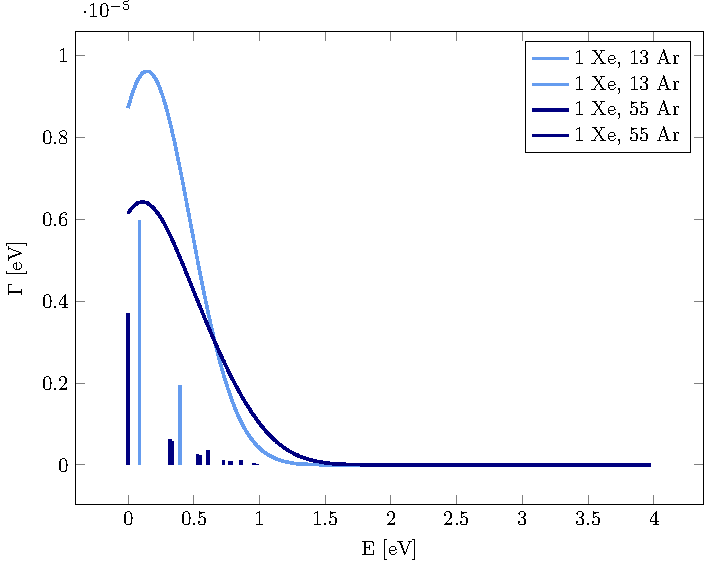
\includegraphics[width=8.0cm]{pics/surf.pdf}\\
 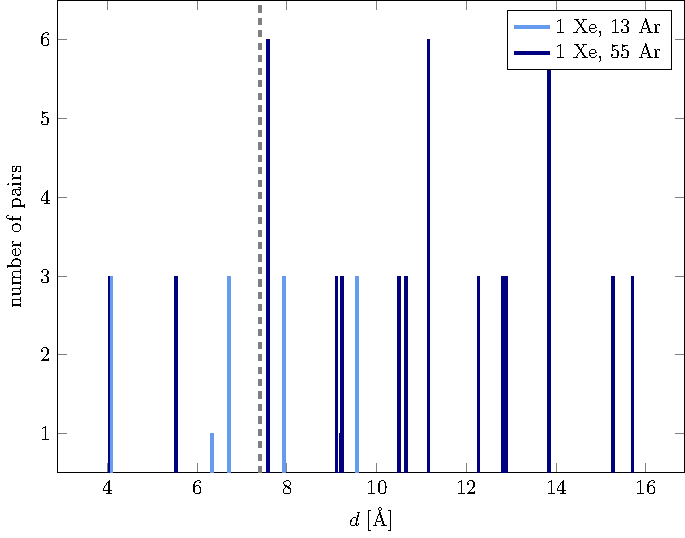
\includegraphics[width=8.0cm]{pics/R_comp.pdf}
 \caption{
 %
 Top panel: Simulated electron emission spectra of an Ar 3s vacancy in 
          argon clusters
          consisting of 13 and 55 atoms, with an additional xenon atom residing
          on top of one of the argon surfaces.
          Bottom panel: Distribution of Ar-Xe distances $d$ in the studied ArXe
          clusters. The ICD channels to final states involving Xe 5p$_{3/2}^{-1}$ and 
          5p$_{1/2}^{-1}$ vacancies open at \unit[7.58]{\AA} and
          \unit[36.00]{\AA}, resp.; the former distance is marked by a vertical dotted line. 
          Only pairs at longer interatomic
          distances contribute to the electron emission spectra.
          Larger Ar-Xe distances, as found in the larger cluster,
          correspond to features at a higher kinetic energy of
          the ICD electron (top panel).}
 \label{figure:surf}
\end{figure}

%In the investigated structures several different aspects have to be
%taken into account which we will discuss separately if possible
%on selected structures.

We will now discuss features of several structures, using selected examples.
First we consider clusters having an argon core of 13 and 55 atoms plus a single xenon
atom on one of the surfaces (see Figure \ref{figure:cluster_3_overview}a
for the structure of clusters with the 55 atoms core).
Secondary electron spectra simulated for these systems are shown in Figure \ref{figure:surf}, top panel.
%two different argon core sizes one consisting
%of 13 and one consisting of 55 atoms with one xenon atom on one of
%the surfaces (see Figure \ref{figure:cluster_3_overview} Panel a)
%for the 55 atom core). The simulated secondary electron spectra are
%shown in Figure \ref{figure:surf} Panel 1.

Because the structures contain only one xenon atom, ETMD(3) is not possible, only ICD is expected. 
%Both spectra show several smaller peaks which
%are convoluted into one single peak with a maximum at
%approximately \unit[0.2]{eV}. 
%In comparison to the 13 argon atoms core
%spectrum t
The spectrum pertaining to the clusters with larger (55 atoms) Ar core shows
signals at higher energies of the secondary electron. These features
can be explained by investigating the Ar-Xe distance distributions
in the clusters, shown
in the lower panel of Figure \ref{figure:surf}. 
Every different value of the atom pair distance
results in a different energy of the secondary electron and only pairs
with a distance of larger than the channel opening distance
(dashed gray line) will contribute
to the spectrum. 
In our model, there is a one-to-one correspondence between interatomic distance $d$ and kinetic energy of the ICD electron.
The larger the interatomic distance, the higher is the
kinetic energy of the secondary electron for a given channel.
%Since the cluster with an Ar core of 55 atoms is larger, and therefore
%contains Ar-Xe pairs with larger distances, its spectrum 
Therefore, the spectrum of the cluster with a 55 atoms core extends to higher energies.
%energies as well.
This relation between ICD energy and cluster size holds true for all cluster structures.
%This explains why the ICD spectrum for larger clusters extends to higher energies, and holds for all cluster structures.

\begin{figure}[ht]
 \centering
 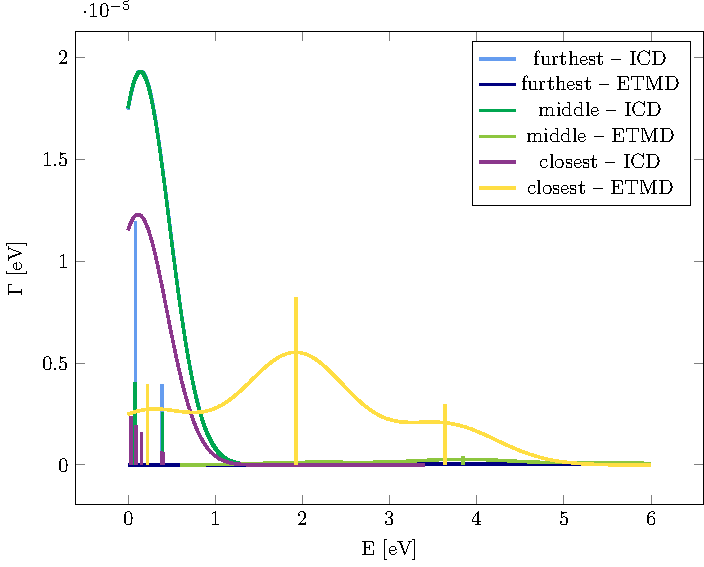
\includegraphics[width=8.5cm]{pics/2tops.pdf}
 \caption{Simulated electron emission spectra of an Ar 3s vacancy in 
          argon clusters consisting of 13
          argon atoms with two additional xenon atoms on top of two different
          argon surfaces. ICD and ETMD spectra are shown for three
          different relative positions of the two xenon atoms. If 
          the xenon atoms are close to each other, an ETMD process is
          clearly visible. In the other two cases the spectra are dominated by
          the ICD spectrum.}
 \label{figure:2tops}
\end{figure}
%
For clusters with more than one xenon atom, also ETMD(3) is possible.
Depending on the positions of the xenon atoms relative to each other and to the Ar core, the spectra are expected to be different.
As an example, we discuss clusters with a core of 13 argon atoms and two xenon atoms on different surfaces. 
Their xenon content is \unit[13.3]{\%} and thus close to the experimental one of \unit[10-12]{\%} for the lowest xenon admixture.
The cluster structures were illustrated in Figure \ref{figure:cluster_2_overview}, simulated spectra are shown in Figure \ref{figure:2tops}.
In all three cases, both ICD and ETMD(3) are energetically allowed. The ICD
spectra do not change qualitatively by adding the second xenon.
%either identical or at least very similar to the ones for
%cluster with a single  consisting of one
%convoluted peak at approximately \unit[0.2]{eV}. 
However, the ETMD(3) spectra
are very sensitive to the relative position of the two xenon atoms.
Two aspects have to be taken into account: an energy shift of the peaks due
to different charge distances $d$ in the final state (i.e. the interatomic Xe-Xe
distance) and the decrease of the decay width with $R^{-6}$, $R$ being the distance
between the electron transfer unit and the xenon atom ionized in the final state.
The larger the distance between the xenon atoms, the higher are the energies
of the secondary electrons. For the case of xenon atoms on argon surfaces
this at the same time means a larger distance between the Ar-Xe pair involved in
the electron transfer and the electron emitting xenon atom. Hence, the
decay widths are smaller. 
Therefore, a
significant contribution from ETMD(3) compared to ICD is only
seen if the two xenon atoms reside on two adjacent
surfaces. 
%{\it Q: Ich verstehe nicht was der n\"chste Satz sagen soll.}
The three energetically separated peaks in the ETMD(3) spectrum pertain to different combinations of the Xe 5p$_j^{-1}$ vacancy states, which have a substantial fine-structure splitting (see Table \ref{tab:valence}). 
%\ref{sec:exp_results}).
%
%The threefold peak structure of the ETMD(3) peak does in contrast to
%the ICD spectrum not stem from different triple structures but from the
%four different decay channels for one triple structure.

\begin{figure}[ht]
 \centering
 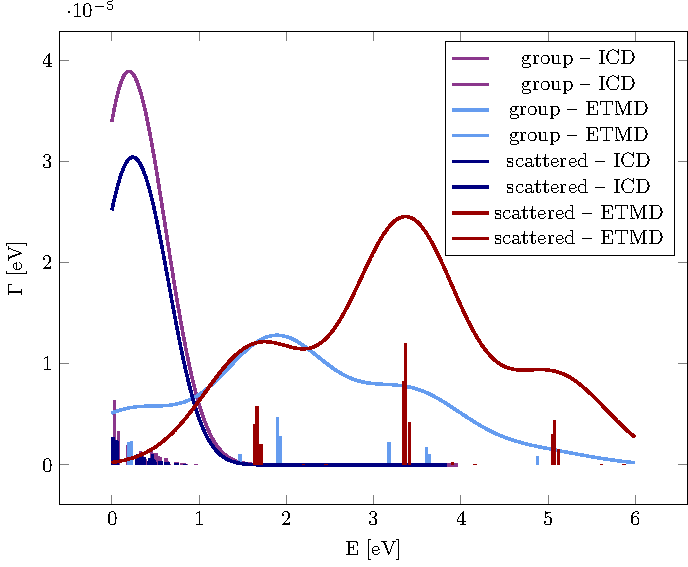
\includegraphics[width=8.5cm]{pics/ar_3_6in.pdf}
 \caption{Same as Figure \protect\ref{figure:2tops}, for clusters consisting of
          55 atoms, 6 out of which are xenon atoms. These are either grouped
          on one side of the cluster (label `group') or evenly distributed
          in the cluster interior (label `scattered').}
 \label{figure:ar_3_6in}
\end{figure}
%
For the 55 atoms clusters, a xenon content of \unit[10--12]{\%}
corresponds to six xenon atoms out of a total of 55 atoms. These can form a connected 
group in one part of the cluster or can be evenly distributed,
as shown in Figures \ref{figure:cluster_3_overview}b and \ref{figure:cluster_3_overview}c. The
ICD and ETMD(3) spectra for these structures are shown in Figure \ref{figure:ar_3_6in}.

For both cases the overall ICD spectra are very similar, and show a maximum at a kinetic energy of approximately \unit[0.3]{eV}. 
In case of grouped xenon atoms, the ICD spectrum extends to slightly higher energies, corresponding to ArXe pairs at slightly larger spatial distances.
A more significant difference is observed in the ETMD(3) spectra. 
The interatomic xenon distance is shorter in clusters, in which the xenon atoms form a connected group.
Hence, the triple structure of the ETMD(3) spectrum is seen at lower kinetic energies. 
Additionally, the probability for an electron
transfer from a xenon to an argon atom decreases exponentially with the
interatomic distance. Therefore, only those xenon atoms which have direct
argon atom neighbours have a significant contribution to the
total decay width, and the total ETMD(3) decay width is lower for the structure with
grouped xenon atoms than for
the structure with evenly distributed xenon atoms (see Table \ref{table:theo_gammas}).

\begin{figure}[ht]
 \centering
 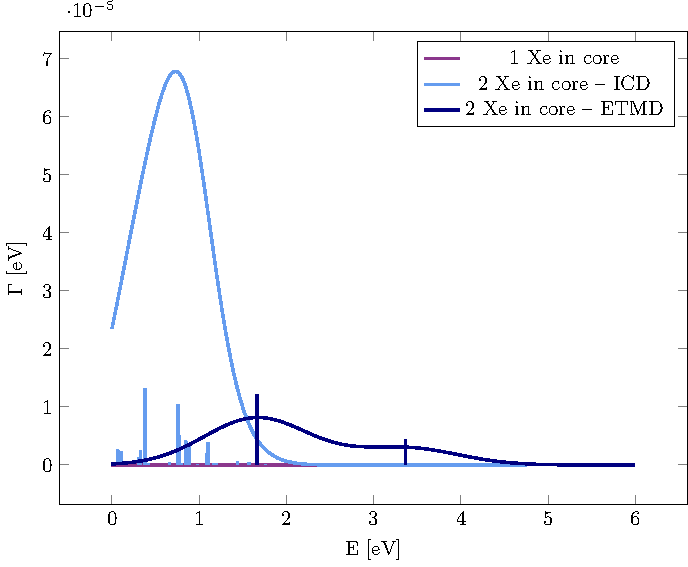
\includegraphics[width=8.5cm]{pics/xe_3_in.pdf}
 \caption{Same as Figure \protect\ref{figure:2tops}, for argon clusters with
          one or two xenon atoms in the core of the cluster (55 atoms total). 
          All ICD and ETMD channels are closed, if the cluster contains only 
          a single xenon atom. For clusters with two xenon atoms
          in the core, the first ICD channel is open for some pairs,
          and additionally ETMD is possible for multiple triples. Due to a
          different distance distribution compared to the clusters with an argon
          core (Figure \protect\ref{figure:2tops}), 
          the ICD peak is shifted to higher kinetic energies.}
 \label{figure:xe_3_in}
\end{figure}
%
For comparison with the previous assumptions of a xenon core surrounded
by argon atoms we investigated clusters of 13 and 55 atoms with one or two
xenon atoms in the core. Some of the corresponding
spectra are shown in Figure \ref{figure:xe_3_in}.

%For the clusters with only one xenon atom in the core and the ionization
%energies used for the simulation of the secondary electron energies
%all ICD channels are closed. Since the cluster contains only one xenon atom,
%an ETMD(3) is not possible. Hence there is no signal to be expected at all.
For a core consisting of two xenon atoms both an ICD and an ETMD(3) spectrum
can be seen. Compared to the cluster structures involving an argon core, the ICD peak is
shifted to higher ICD electron energies. 
Additionally, the ICD and ETMD(3) spectra overlap.
For ETMD(3), only three of the four different decay channels are
energetically allowed.

\begin{figure}[ht]
 \centering
 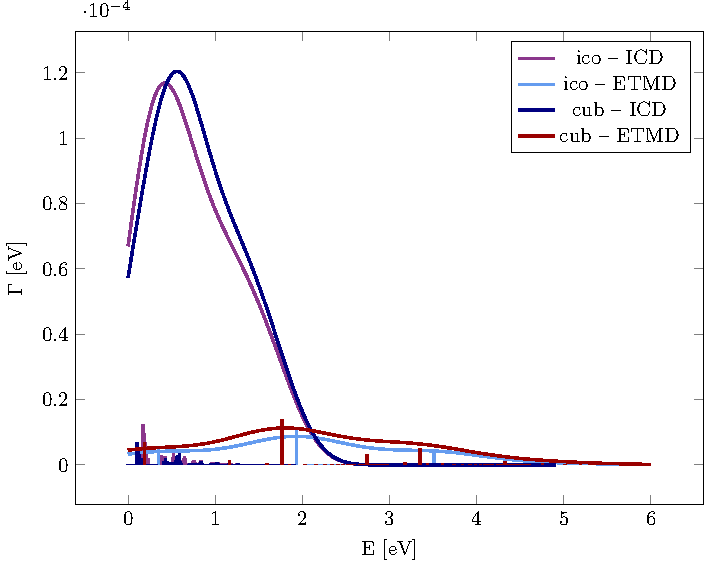
\includegraphics[width=8.5cm]{pics/c6l5.pdf}
 \caption{Same as Figure \protect\ref{figure:2tops},
          for a large cluster consisting
          of a xenon core of 561 atoms surrounded by five complete layers of
          argon atoms (Xe content: 14.5\,\%) for both an icosahedral and
          cuboctahedral basic structure.
          The ICD and ETMD peak overlap such that the ETMD peak
          is unlikely to be visible.}
 \label{figure:xe_6_lay5}
\end{figure}
%
In the first experiments very large argon-xenon clusters of 
$\approx 4380$ atoms with a xenon content of \unit[19]{\%}
were measured,\cite{Mucke_phd}
which we in one example approximate by a cluster consisting of 561 xenon
atoms surrounded
by five layers of argon atoms (3871 atoms in total). In order to take the
better stabilization of charges in larger clusters into account, the
ionization energies of the XL clusters (see Table \ref{tab:valence})
were used.
The spectra are shown in 
Figure \ref{figure:xe_6_lay5}.

Compared to the small clusters with a xenon core in Figure \ref{figure:xe_3_in}
the ICD peak is broadened and shifted to higher ICD electron energies which is
expected due to the larger interatomic Ar-Xe distances in the large cluster and
the better stabilization of charges, which is relevant mostly for the final state, but also the initial state.
The ETMD(3) peak is shifted to slightly higher energies as well. This allows opening of the
fourth decay channel, pertaining to Xe 5p$_{1/2}^{-1}$ Ar 3p$_{1/2}^{-1}$ final states.

We also note that the percentage of decay via ICD is practically
independent of the Xe content for large clusters with a Xe core, Ar shell structure.
This can be expected, as both decay processes are most pronounced for the
atoms in the interface region of the xenon core and the argon shell.
The ETMD(3), depending on the electron transfer from one xenon atom to the
initially ionized argon atom, and hence on the corresponding orbital overlap,
is purely an interface effect that involves the argon atoms with direct xenon
neighbours, and the two xenon layers closest to the argon shell.
The ICD has a stronger long range character, due to which the description
of decays with partners of at least twice the smallest channel opening
distance is necessary for clusters. However, the bigger the clusters are,
the more homogeneous does the interface region become for clusters of
different sizes. This manifests itself in the distribution of relevant
Ar-Xe pair distances (compare Figure \ref{figure:surf}, lower panel).
As a consequence, the ICD spectra of two large clusters of different size
hardly differ.

All these results neglect the effect of nuclear dynamics, which might
affect the spectra. Possible reasons are distance dependend channel closings
and openings,
a different distribution of interatomic distances due to vibrations
and their different impact on
the ICD and the ETMD(3). E.g., for the ICD in the neon dimer, the treatment of
nuclear dynamics increases the decay width by approximately a factor 2
\cite{Schnorr15}.
However, the atomic displacement can be expected to be by far less severe
in clusters than in dimers or trimers. Additionally, 
the elongation of one interatomic distance in a cluster
automatically results in
the shortening of a different interatomic distance, which will reduce
the overall effect. Therefore, there will be a broader spectrum charges in the
final state $d$ resulting in a broadening of the peak. This was taken into
account by folding the stick spectrum with Gaussians with a width of
\unit[300]{meV} and \unit[600]{meV} for the ICD and ETMD(3), respectively.
While the width of the ICD peaks was estimated from the potential energy
surface of the ArXe dimer, the situation is more complex in case of the ETMD(3)
with three degrees of freedom involved. It was therefore guessed to be twice the
width of the ICD peak.

The channel closing due to shortening of the interatomic distance is not
relevant for the ETMD(3) process in the ArXe clusters, treated in this work,
because this would require unnaturally short interatomic distances.
However, for the ICD it might result in a lower number of pairs with open
decay channels and hence decrease the decay width. Since the folded peaks
are constituted from several pairs of different distances, it would result
in a slight peak shift to higher energies of the combined peak at lowest energy.
For a more detailed discussion of nculear dynamics for the ICD in dimers vs.
in clusters see Ref. \citenum{fasshauernjp}






\clearpage
